\documentclass[11pt,a4paper]{article}
%bvbfbvbv
\usepackage{fullpage}
\let\proof\relax
\let\endproof\relax
\usepackage{amsmath,amsthm,amssymb,amsfonts,color,bm}
\usepackage[pdftex]{graphicx}
%\usepackage{cite}
\usepackage{mathtools}
\usepackage{physics}
\let\norm\relax
\DeclarePairedDelimiter{\norm}{\lVert}{\rVert}
\newcommand{\pushright}[1]{\ifmeasuring@#1\else\omit\hfill$\displaystyle#1$\fi\ignorespaces}
\newcommand{\pushleft}[1]{\ifmeasuring@#1\else\omit$\displaystyle#1$\hfill\fi\ignorespaces}
\newcommand{\cu}[1]{\mathbf{#1}}
\newcommand{\tash}[2]{\frac{\partial #1}{\partial #2}}
\newcommand{\tashh}[2]{\frac{\partial^2 #1}{\partial {#2}^2}}
\newcommand{\innerp}[2]{\langle{#1}, {#2}\rangle}

\newcommand{\bracket}[2]{\left\{\begin{matrix}
		#1\\
		#2
	\end{matrix}\right.}
\newcommand{\easytwo}[2]{\begin{bmatrix}
		#1\\ 
		#2
\end{bmatrix}}
\newcommand{\easyfour}[4]{\begin{bmatrix}
		#1& #2\\ 
		#3& #4
\end{bmatrix}}
\newcommand{\easynine}[9]{\begin{bmatrix}
		#1& #2& #3\\ 
		#4& #5& #6\\
		#7& #8& #9
\end{bmatrix}}
\newcommand{\fastmatrix}[1]{\begin{pmatrix}#1\end{pmatrix}}

%%% Functions

\DeclareMathOperator*{\argmin}{arg\,min}  % Argmin
\DeclareMathOperator*{\argmax}{arg\,max}  % Argmax

%\DeclareMathOperator\erf{erf} % Standard error function

%%% Probability

\newcommand{\expec}{\mathbb{E}}           % Expectation
\newcommand{\cov}{\operatorname{Cov}}     % Covariance
\newcommand{\varr}{\operatorname{Var}}     % Variance
\newcommand{\gauss}{\mathcal{N}}          % Gaussian distribution

%%% Number sets

\newcommand{\R}{\mathbb{R}} % Set of real numbers
\newcommand{\Q}{\mathbb{Q}} % Set of rational numbers
\newcommand{\N}{\mathbb{N}} % Set of natural numbers
\newcommand{\Z}{\mathbb{Z}} % Set of integers

%%% Standard constants and objects
\DeclareMathOperator{\neper}{e} % Exponential constant

%% Linear algebra operations
\newcommand{\transpose}{\mathsf{T}}         % Transpose of a matrix
%\newcommand{\trace}{\operatorname{tr}}      % Matrix trace
\newcommand{\adj}{\operatorname{adj}}       % Matrix adjugate
\newcommand{\diag}{\operatorname{diag}}     % Diagonal matrix
%\newcommand{\rank}{\operatorname{rank}}     % rank of a matrix
\newcommand{\Hess}{\operatorname{Hess}}     % Hessian matrix
\newcommand{\lspan}{\operatorname{span}}    % linear span
\newcommand{\mineig}{\lambda_{\text{min}}}  % Minimal eigenvalue
\newcommand{\maxeig}{\lambda_{\text{max}}}  % Maximal eigenvalue

%% Complement

% \newtheorem{theorem}{Theorem}
\usepackage{amsfonts}
\usepackage{amsmath}
\usepackage{amssymb}
\usepackage{microtype}
\usepackage{fouriernc}
\usepackage{graphicx}
\usepackage{times}
\usepackage{url}
\usepackage{listings}
\usepackage{color}
\usepackage{mathrsfs}
\usepackage{listings}
\usepackage{autobreak}
\usepackage{cite}
\definecolor{mygreen}{rgb}{0,0.4,0}
\definecolor{myblue}{rgb}{0,0,0.4}
\lstset{language=Matlab,
  basicstyle=\scriptsize\ttfamily,
  keywordstyle=\bfseries\color{black},
  commentstyle=\itshape\color{red},
  identifierstyle=\color{myblue},
  stringstyle=\color{mygreen},
  }
\title{Notes on Neural Networks based on primal-dual splitting method }
\author{Rui, Zheng}

\begin{document}
\maketitle

\tableofcontents
\section{Possible paper production}
Ordered by priority from high to low
\begin{itemize}
	\item Training NN with ADMM (Prime-Dual); 
	\item Train CapsuleNet with ADMM
	\item Spectro-temporal Layer with ADMM
	\item CSC with ADMM
\end{itemize}
\section{Introduction}
Deep neural networks (DNNs) have  have been used to solve a wide variety of applications such as image classification, object recognition, natural language processing, etc. Although, gradient based search techniques such as backpropagation
are currently the most widely used optimization techniques for training neural networks, it has been shown that these gradient techniques are severely limited in their ability to computational efficiency. 
\section{Problem formulation}
Consider a dataset $\mathcal{D}(\cu{X}, \cu{y})$ of $n$ observations where $\mathbf{X}$ denotes an input matrix (covariates) of dimension $D_x \times n$ and $\mathbf{y}$ denotes the scalar output (or target) variable.  Given this training dataset,  we wish to make predictions for new inputs $\mathbf{x}^*$. A typical objective function to learn a DNNs with $L$ layers has the
form 
\begin{equation}
J(\cu{w}; \mathcal{D}) = L(\cu{w}; \mathcal{D}) + \lambda \phi (\cu{w})
\end{equation}. 
Here, the loss functions $L(\cu{w}; \mathcal{D})$ are usually MSE or crossentropy:
For 1) mean square error (MSE), the above equation generalizes to:

\begin{equation}
\begin{split}
\label{eq:objective_mse}
J(\cu{w}; \cu{X}, \cu{y}) = \frac{1}{2N}\norm{\cu{y} - f(\cu{w}, \cu{X})}^2 + \lambda \phi(\cu{w}) \\
= \frac{1}{2N}\norm{\cu{y} - f(\cu{w}, \cu{X})}^2 + \lambda \| \cu{w} \|_1
\end{split}
\end{equation}
where $f$ is the prediction function, $\mathbf{w}$ is the parameter we optimize,  and $\lambda$ is the constant. 

For 2) crossentropy:
\begin{equation}
J(\cu{w}; \cu{X}, \cu{y}) = \sum^N_{i=1}(y_i\log f(\cu{w},\cu{x}) + (1-y_i)\log (1-f(\cu{w}, \cu{x}))) + \lambda \phi(\cu{w})
\end{equation}
where $\lambda \phi(\cu{w})$ can be any regularizers (L1, L2 etc.), and $f(\cdot)$ is network function. 

The aim here is to find the optimize values weights $\mathbf{w}$ of neural network to minimize the objective function. 

\subsection{One Example}
For a simplest NN example. Here we will use the notation: $\cu{x}\in \mathbb{R}^5: \cu{x} = \{x_1, x_2, ..., x_5\}$ and $y: y\in \mathbb{R}$ as the pair of data for training; $w^l_{ij}$ denotes the weight that connects $i$-th neuron on $(l-1)$-th layer and $j$-th neuron on $l$-th layer; $\sigma_l(\cdot)$ is the activation function for $l$-th layer; $o^l_i$ is the output from the $i$-th neuron of $l$-th layer; $Out$ is the output of the neural network (last neuron): 

\begin{figure}[h!]
	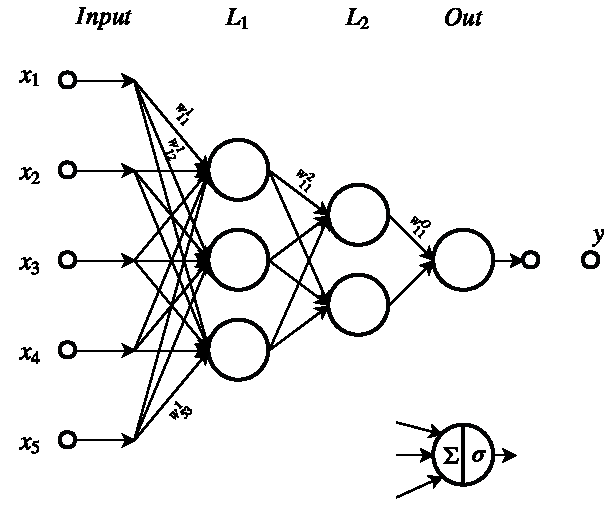
\includegraphics[scale=0.75]{figs/nn}
	\centering
\end{figure}

The loss is:

\begin{equation}
J(\cu{W}; \cu{x}, y) = \frac{1}{2} (Out_{\cu{w},\cu{x}} - y)^2 + \text{regularizer on } \cu{w}
\end{equation}

Let us show some forward example of it. Take output $Out$:
\begin{align}
Out &= \sigma_3(o^2_1w^3_{11} + o^2_2w^3_{21} + b^3)\\
&= \sigma_3(\cu{o}^2\cu{w}^3 + b_3)\\
&= \sigma_3(\Sigma^3_1)
\end{align}
where $\cu{o}^2 = [o^2_1, o^2_2]$, $\cu{w}^3 = [w^3_{11}, w^3_{21}]^T$ and $\Sigma^3_1 = \cu{o}^2\cu{w}^3 + b_3$.
Let us continue for $o^2_1$ and $o^2_2$:
\begin{align}
o^2_1 &= \sigma_2(o^1_1w^2_{11} + o^1_2w^2_{21} + o^1_3w^2_{31} + b^2_1)\\
&= \sigma_2(\Sigma^2_1)\\
o^2_2 &= \sigma_2(o^1_1w^2_{12} + o^1_2w^2_{22} + o^1_3w^2_{32} + b^2_2)\\
&= \sigma_2(\Sigma^2_2)\\
\cu{o}^2 &= \sigma_2(\cu{o}^1\cu{w}^2 + \cu{b}^2)
\end{align}
where $\cu{o}^1 = [o^1_1, o^1_2, o^1_3]$ and $\cu{w}^2 = \begin{bmatrix}
w^2_{11} & w^2_{21} & w^2_{31}\\
w^2_{12} & w^2_{22} & w^2_{32}
\end{bmatrix}^T$. and $\cu{o}^1 = \sigma_1(\cu{x}\cu{w}^1 + \cu{b}^1)$. 

In traditional approach, we need to derive the gradient of the loss w.r.t each weight i.e.:

\begin{equation}
\tash{J(\cu{W}; \cu{x}, y)}{w^l_{ij}}
\end{equation}

Those gradient can be efficiently obtained by backpropogation (BP). For simplicity, BP not discussed here. 

If we use SGD, the update of weight is just: $w^l_{ij}(k+1) = w^l_{ij}(k) + \eta \tash{J(\cu{W}; \cu{x}, y)}{w^l_{ij}}$.

Based on SGD, we consider using ADMM to solve the objective function. 
%So what about updating the weight using ADMM or Prime-Dual? The only motivation for doing this is that we can use fancier regularizers %(e.g. $\norm{\bm{\Omega} \cu{w}}$)?


\section{Spectro-temporal layer}

Considering an LTI system:

\begin{equation}
\begin{split}
\cu{x}_k & = \cu{A}\cu{x}_{k-1} + \cu{q}, \hfill \cu{q}_k\sim\mathcal{N}(\cu{0},\cu{Q})\\
y_k &= \cu{H}\cu{x}_k + r_k, \hfill r_k\sim\mathcal{N}(0, R)
\end{split}
\label{equ:osc-model}
\end{equation}
where $\cu{A}$, $\cu{Q}$ and $\cu{H}$ are defined as:
\begin{align}
\cu{A} &= \begin{bmatrix}
1 & & &\\
& \cu{A}^1_k & &\\
& & \ddots &\\
& & & \cu{A}^M_k
\end{bmatrix}\\
\cu{Q} &= \begin{bmatrix}
qb \Delta t & & &\\
& \cu{Q}^1_k & & \\
& & \ddots & \\
& & & \cu{Q}^M_k
\end{bmatrix}\\
\cu{H} &= [1, \cu{H}^1, \ldots, \cu{H}^M] = [1 1 0 1 0, \ldots, 1 0]
\label{equ:osc-a-q-h}
\end{align}  

where $\cu{A}^j_k$ and $\cu{Q}^j_k$ are given in closed form:
\begin{align}
\cu{A}^j_k &= \exp(\cu{F}_j\Delta t)\\
&= \begin{bmatrix}
\cos (2\pi f_j\Delta t) & -\sin (2\pi f_j\Delta t)\\
\sin (2\pi f_j\Delta t) & \cos (2\pi f_j\Delta t)
\end{bmatrix}\exp(-\Delta t \lambda_j)\\
\cu{Q}^j_k &= \int_0^{\Delta t} \exp(\cu{F}_j(\Delta t-s)) \cu{L}\cu{Q}^j_k\cu{L}^\top \exp(\cu{F}_j(\Delta t-s))^\top ds\\
&= \frac{Q^j_k}{2\lambda^j}(1 - \exp(-2\Delta t \lambda_j)) \cu{I}
\label{equ:osc-solve}
\end{align}

We can use Kalman filter to easily estimate $\cu{x}_k$. 

However, the point of spectro-temporal layer is that we set $\cu{A}$ and $\cu{Q}$ are paramiterized by \textbf{trainable} weight $\cu{w}$. 

\begin{equation}
\begin{split}
\cu{x}_k & = \cu{A}(\cu{w})\cu{x}_{k-1} + \cu{q}, \hfill \cu{q}_k\sim\mathcal{N}(\cu{0},\cu{Q}(\cu{w}))\\
y_k &= \cu{H}\cu{x}_k + r_k, \hfill r_k\sim\mathcal{N}(0, R)
\end{split}
\label{equ:osc-model}
\end{equation}

We put a signal $y$ as input of this layer. After Kalman estimation, it outputs a spectrogram (image) $\cu{X}$, we then feed that $\cu{X}$ into NN to classify. Because $\cu{A}$ and $\cu{Q}$ are trainable for NN, thus just optimize that NN loss function, but the computational cost is very expensive. 

\section{ADMM solver for MSE}
We consider the original optimization problem~\eqref{eq:objective_mse}. Firstly, we introduce an auxiliary variable $\mathbf{V}$, and have the following constrained problem  
\begin{equation}\label{eq:admm}
\begin{split}
\min_{x} &\frac{1}{2} \| y - H \, x \|^2_{R^{-1}}
   + \frac{1}{2} \| \Psi \, x - m \|^2_{Q^{-1}} 
   + \lambda \|\Omega\, x \|_1  \\
\mathrm{s.t.}\ & v = \Omega\,x . 
\end{split}
\end{equation}

\begin{equation}
\begin{split}
\label{eq:objective_mse}
\min_{W} &\frac{1}{2} \sum_{n=1}^N \norm{\cu{y}_n - f(\cu{W}, \cu{x})}^2 + \lambda \| \cu{V} \|_1 \\
\mathrm{s.t.}\ & \mathbf{V} = \mathbf{W} .
\end{split}
\end{equation}

Then, Let $\mathcal{L_\rho}(x,v;\eta)$ be the augmented Lagrangian function of~Eq.~\eqref{eq:objective_mse} which is defined as follows
\begin{equation}\label{eq:Lagrangian_func}
\begin{split}
\begin{aligned}
\mathcal{L_\rho}(\mathbf{W},\mathbf{V};\bm\eta) \triangleq 
 \frac{1}{2} \sum_{n=1}^N \norm{\cu{y}_n - f(\cu{W}, \cu{x})}^2 + \lambda \| \cu{V} \|_1 
+ \langle \mathbf{V}- \mathbf{W} ,\bm\eta\rangle
+ \frac{\rho}{2}\left \| \mathbf{V}- \mathbf{W}\right \|^2
\end{aligned}
\end{split}
\end{equation}
The solution of~\eqref{eq:Lagrangian_func} can be obtained by the following steps \cite{Boyd2011ADMM}:
\begin{equation}
\begin{split}
\mathbf{W}^{k+1} &:= \arg\min_{\mathbf{W}} \mathcal{L_\rho} (\mathbf{W},\mathbf{V}^k;\bm\eta^k) \\
\mathbf{V}^{k+1} &:= \arg\min_{\mathbf{W}} \mathcal{L_\rho} (\mathbf{W}^{k+1},\mathbf{V};\bm\eta^k) \\
\bm\eta^{k+1}    &:= \bm\eta^{k} + \rho (\mathbf{V}^{k+1} - \mathbf{W}^{k+1})
\end{split}
\end{equation}

\begin{enumerate}
\item Input: $ \mathbf{V}^0$, $\bm\eta^0$, $\rho$,
\item Loop: For $k=1,2,\cdots$ until termination criteria are met.
\begin{itemize}
\item Calculate $x^k $ by solving: 
\begin{equation}
\label{eq:w_update}
\begin{split}
\
\mathbf{W}^{k+1} &= \arg \min_{\mathbf{W}} \ \mathcal{L_\rho} (\mathbf{W},\mathbf{V}^k;\bm\eta^k) \\
        &= \arg \min_{\mathbf{W}}  \   
        \frac{1}{2} \sum_{n=1}^N \norm{\cu{y}_n - f(\cu{W}, \cu{x})}^2 + 
          + \frac{\rho}{2} \left\| \mathbf{V} - \mathbf{W} + \bm\eta \right\|^2 
\end{split}
\end{equation}
Eq.~\ref{eq:w_update} has the close-form expression. We could use RTS smoother to solve the problem~\eqref{eq:w_update} 

\item Calculate $\mathbf{V}^k $ by solving: 
\begin{equation}
\begin{split}
\mathbf{V}^{k+1} &= \arg \min_\mathbf{V} \ \mathcal{L_\rho}(\mathbf{W}^{k+1},\mathbf{V};\bm\eta^k)  \\
&= \lambda \left \| \mathbf{V} \right \|_1+\frac{\rho}{2}\left \| \mathbf{V}- \mathbf{W}^{k+1} + \bm\eta^{k}\right \|^2 \\
&= \operatorname{sign}(\mathbf{W}^{k+1} + \bm\eta^k/\rho) \circ \operatorname{max} (|\Omega x^{k+1} + \eta^k/\rho|-{\lambda}/{\rho},0 )
\end{split}
\end{equation}
where $\operatorname{sign}$ represents the signum function, and $\circ$ is the pointwise product. 
\item Calculate $\eta^k $ by solving:
\begin{equation}
\begin{split} 
\eta^{k+1}= \eta^{k}+ \rho (\Omega\,x^{k+1} -v^{k+1} )
\end{split}
\end{equation}
\end{itemize}
\item Output: $x^{k+1}$
\end{enumerate}




\section{Matlab example}
%\lstinputlisting{example/***.m} 

\bibliography{note_refs}{}
\bibliographystyle{plain}
\end{document}
